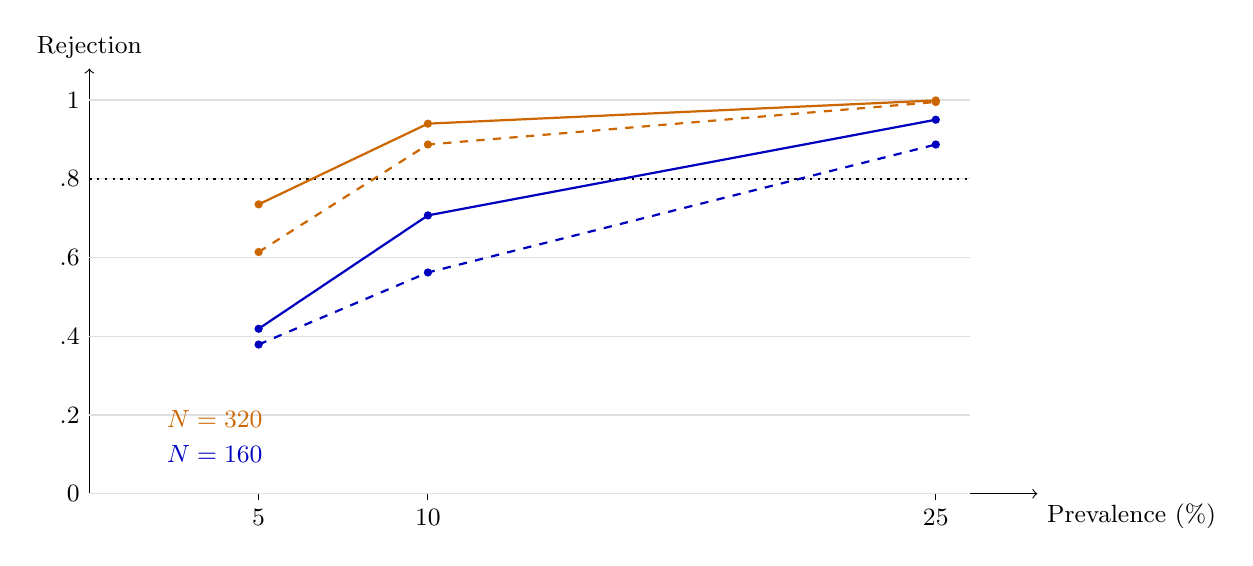
\begin{tikzpicture}[x=0.43cm,y=5cm,font=\small]
\draw[->] (0,0)--(28,0) node[below right] {Prevalence (\%)};
\draw[->] (0,0)--(0,1.08) node[above,align=center] {Rejection};
\foreach \y in {0,.2,.4,.6,.8,1}{\draw[gray!25] (0,\y)--(26,\y);\node[left] at (0,\y) {\y};}
\foreach \x in {5,10,25}{\draw (\x,0)--++(0,-.015);\node[below] at (\x,-.015) {\x};}
\draw[dotted,thick] (0,.8)--(26,.8);
\draw[thick,blue!75!black] plot coordinates {(5,0.419)(10,0.707)(25,0.950)};
\fill[blue!75!black] (5,0.419) circle[radius=1.5pt];
\fill[blue!75!black] (10,0.707) circle[radius=1.5pt];
\fill[blue!75!black] (25,0.950) circle[radius=1.5pt];
\draw[thick,blue!75!black,dashed] plot coordinates {(5,0.379)(10,0.562)(25,0.887)};
\fill[blue!75!black] (5,0.379) circle[radius=1.5pt];
\fill[blue!75!black] (10,0.562) circle[radius=1.5pt];
\fill[blue!75!black] (25,0.887) circle[radius=1.5pt];
\draw[thick,orange!80!black] plot coordinates {(5,0.735)(10,0.940)(25,0.999)};
\fill[orange!80!black] (5,0.735) circle[radius=1.5pt];
\fill[orange!80!black] (10,0.940) circle[radius=1.5pt];
\fill[orange!80!black] (25,0.999) circle[radius=1.5pt];
\draw[thick,orange!80!black,dashed] plot coordinates {(5,0.614)(10,0.887)(25,0.995)};
\fill[orange!80!black] (5,0.614) circle[radius=1.5pt];
\fill[orange!80!black] (10,0.887) circle[radius=1.5pt];
\fill[orange!80!black] (25,0.995) circle[radius=1.5pt];
\node[anchor=west,blue!75!black] at (2,.10) {$N=160$};
\node[anchor=west,orange!80!black] at (2,.19) {$N=320$};
\end{tikzpicture}
